% main.tex
% Fichero principal de transparencias (incluye a todos los demás).

% Compilar a .pdf con LaTeX (pdflatex)
% Es necesario instalar Beamer (paquete latex-beamer en Debian)
%

% Gráficos:
% Los gráficos pueden suministrarse en PNG, JPG, TIF, PDF, MPS
% Los EPS deben convertirse a PDF (usar epstopdf)
%
\documentclass[17pt,aspectratio=169,hyperref=pdfusetitle]{beamer}
\usetheme[orchid]{Hannover}
\beamertemplatenavigationsymbolsempty
\setbeamertemplate{headline}{}
\useoutertheme{infolines}

\usepackage[spanish]{babel}
\usepackage[utf8]{inputenc}
\usepackage{graphics}
%\usepackage{amssymb} % Simbolos matematicos
%\usepackage[pdfusetitle]{hyperref}

\usepackage{chronosys}

%% two slides per page
%\usepackage{pgfpages}
%\pgfpagesuselayout{2 on 1}[a4paper,border shrink=5mm]

\newcommand\YUGE{\fontsize{48}{60}\selectfont}

\newcommand{\secimage}{figs/bookpages}
\AtBeginSection[]
{
  {
    \usebackgroundtemplate{\includegraphics[width=\paperwidth,height=\paperheight]{\secimage}}
    \begin{frame}<beamer>

      \begin{center}
        {\YUGE\bf\insertsection}
      \end{center}
    \end{frame}
  }
  \renewcommand{\secimage}{figs/bookpages}
}


\title[Can software be healthy?]{Can software be healthy?}
%\subtitle{}
\author[Jesus M. Gonzalez-Barahona]{Jesus M. Gonzalez-Barahona}
\institute[URJC]{Universidad Rey Juan Carlos \\
  @jgbarah ~~~~~ \url{http://jgbarah.github.io/presentations}}

\date[SoHeal 2019]{SoHeal 2019 \\ Montreal (Canada), May 28th 2019}

\begin{document}

%\begin{frame}[label=firstframe]
\begin{frame}
  \maketitle
\end{frame}


\begin{frame}

  {\em
    \begin{center}
      %\begin{quote}
      Health, \\
      what is health? \\
      Can anyone be healthy \\
      at all? \\
      %\end{quote}
    \end{center}
  }
\end{frame}


%%%%%%%%%%%%%%%%%%%%%%%%%%%%%%%%%%%%%%%%%%%%%%%%%%%%%%%%%%%%%%%%
%%%%%%%%%%%%%%%%%%%%%%%%%%%%%%%%%%%%%%%%%%%%%%%%%%%%%%%%%%%%%%%%
% lista de temas                                               %
%%%%%%%%%%%%%%%%%%%%%%%%%%%%%%%%%%%%%%%%%%%%%%%%%%%%%%%%%%%%%%%%
%%%%%%%%%%%%%%%%%%%%%%%%%%%%%%%%%%%%%%%%%%%%%%%%%%%%%%%%%%%%%%%%


\definecolor{lightviolet}{HTML}{F4AFF4}
\definecolor{lightorange}{HTML}{FFA17F}
\definecolor{lightgreen}{HTML}{98FB98}
\definecolor{lightred}{HTML}{FF5C5C}
\definecolor{lightblue}{HTML}{89AFCF}
\definecolor{lightbrown}{HTML}{B58868}

%%-----------------------------------------
%%-----------------------------------------
\section{What do we want?}

%%-----------------------------------------
\begin{frame}[fragile]

  {\em
      \begin{quote}
      Speaker: What do we want? \\
      Crowd: Patience! \\
      Speaker: When do we want it? \\
      Crowd: Right now!!! \\
      \end{quote}
  }

  \begin{flushright}
    {\small Adapted from a well known joke \\
    by Eugenio (Spanish humorist). \\}
  \end{flushright}
\end{frame}

%%-----------------------------------------
\begin{frame}[fragile]
  \frametitle{The theory}

  {\em
    \begin{quote}
      Software should behave \\
      according to requirements, \\
      be cheap to maintain, \\
      be easy to use, \\
      have good performance, \\
      ... \\
      \end{quote}
  }

  {\large
  ``We want software of good quality''
  }
\end{frame}

%%-----------------------------------------
\begin{frame}[fragile]
  \frametitle{The practice}

  In most cases...
  
  \begin{itemize}
  \item Functionality: shallow verification
  \item Requirements: from nonexistent to incomplete
  \item Maintainability: very expensive
  \item Usability: many facets
  \item Performance: only a relative target
  \end{itemize}

  ``Good enough'', depending on the stakeholder
  
\end{frame}

%%-----------------------------------------
%%-----------------------------------------
\section{Improving quality}

%%-----------------------------------------
\begin{frame}[fragile]
  \frametitle{The quest for quality}

  ``Traditional'' approach in software engineering:
  
  \begin{itemize}
  \item Product quality \\
    (ISO 9126, CISQ)
  \item Process quality \\
    (ISO 9001, CMM)
  \end{itemize}

  Follow the rules, increase quality
\end{frame}


%% %%-----------------------------------------
%% \begin{frame}[fragile]
%%   \frametitle{If you know ``the right way to do it''}

%%   \begin{itemize}
%%   \item Define characteristics of processes \\
%%     Process maturity models \\
%%     Example: CMM
%%   \item Define characteristics of code \\
%%     Software quality models \\
%%     Example: CISQ
%%   \end{itemize}
%% \end{frame}

%%-----------------------------------------
\begin{frame}[fragile]
  \frametitle{CISQ (code) quality model}
  
  \begin{itemize}
  \item reliability
  \item efficiency
  \item security
  \item maintainability
  \end{itemize}

  \begin{flushright}
    \url{https://www.it-cisq.org}
  \end{flushright}
  
\end{frame}

%%-----------------------------------------
\begin{frame}[fragile]
  \frametitle{CISQ (code) quality model}

  \begin{center}
  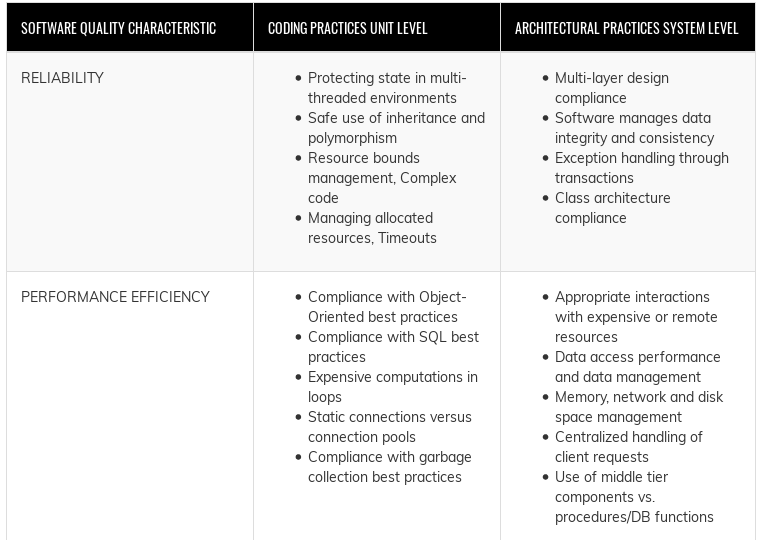
\includegraphics[height=7cm]{figs/cisq}
  \end{center}  
  
\end{frame}

  
%% %%-----------------------------------------
%% \begin{frame}[fragile]
%%   \frametitle{CMM development model}
  
%%   \begin{itemize}
%%   \item policy
%%   \item standard
%%   \item process
%%   \item procedure
%%   \item level overview
%%   \end{itemize}

%%   \begin{flushright}
%%     {\footnotesize
%%     Paulk, Weber, Curtis, Chrissis, Beth ``Capability Maturity Model for Software (Version 1.1)'' Software Engineering Institute, Carnegie Mellon University. CMU/SEI-93-TR-024, Feb 1993 \\
%%     \url{http://www.sei.cmu.edu/library/abstracts/reports/93tr024.cfm}
%%     }
%%   \end{flushright}
  
%% \end{frame}

%%-----------------------------------------
%%-----------------------------------------
\section{Measuring quality}

%%-----------------------------------------
\begin{frame}[fragile]
  \frametitle{There are other motivations}

  \begin{flushright}
  What if the focus is ``knowing'' \\
  instead of ``improving'' \\
  \end{flushright}
  
  \begin{itemize}
  \item comparison
  \item tracking
  \item self-awareness
  \end{itemize}
\end{frame}

%%-----------------------------------------
\begin{frame}[fragile]
  \frametitle{There are other subjects}

  \begin{flushright}
    What if the people \\
    are also important? \\
  \end{flushright}
  
  \begin{itemize}
  \item the builders
  \item the evaluators
  \end{itemize}
\end{frame}


%%-----------------------------------------
\begin{frame}[fragile]
  \frametitle{The builders}

  Specially important in FOSS:

  \begin{itemize}
  \item diverse people working together
  \item different motivations, agendas...
  \item the sense of community
  \end{itemize}
    
\end{frame}

%%-----------------------------------------
\begin{frame}[fragile]
  \frametitle{The evaluators}

  \begin{center}
  Different goals / interests

  mean

  different definitions of ``good''
  \end{center}
    
\end{frame}

%%-----------------------------------------
\begin{frame}[fragile]
  \frametitle{And we still have the context...}

  Software is not used in a vacuum:

  \begin{itemize}
  \item legalese
  \item support
  \item economy
  \item ecosystem
  \item ...
  \end{itemize}
\end{frame}


%%-----------------------------------------
%%-----------------------------------------
\section{A bit of history}

%%-----------------------------------------
\begin{frame}[fragile]
  \frametitle{OpenBRR}

  
  \begin{center}
  
\includegraphics[height=2cm]{figs/openbrr}

  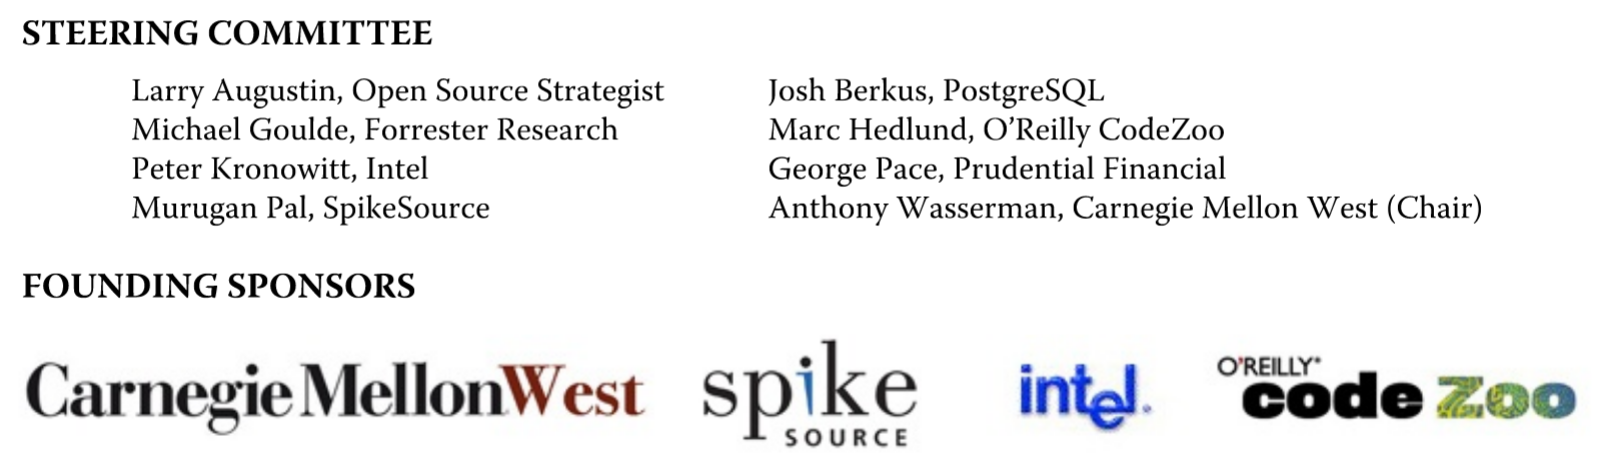
\includegraphics[height=3.5cm]{figs/openbrr-authors}
  \end{center}  
  
\end{frame}

%%-----------------------------------------
\begin{frame}[fragile]
  \frametitle{OpenBRR}

  
  \begin{center}
  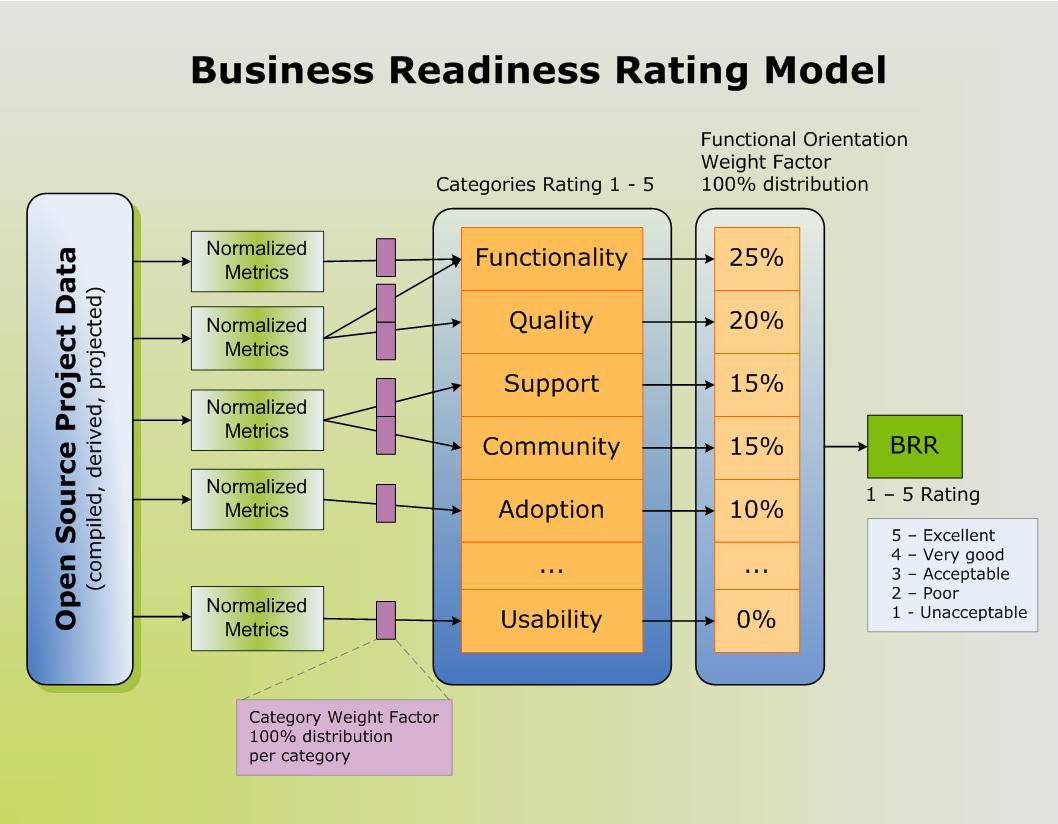
\includegraphics[height=7cm]{figs/openbrr-model}
  \end{center}  
  
\end{frame}


%% %%-----------------------------------------
%% \begin{frame}[fragile]
%%   \frametitle{Qualoss}
  
%% \end{frame}

%%-----------------------------------------
\begin{frame}[fragile]
  \frametitle{QSOS}

  \begin{center}
  
\includegraphics[height=5.5cm]{figs/qsos}
  \end{center}  

\end{frame}


%%-----------------------------------------
\begin{frame}[fragile]
  \frametitle{QSOS}

  \begin{center}
  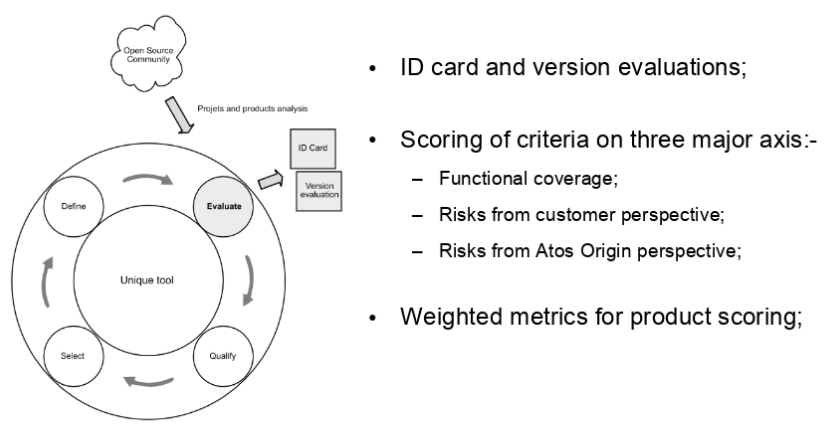
\includegraphics[height=6cm]{figs/qsos-model}
  \end{center}  

\end{frame}


%%-----------------------------------------
\begin{frame}[fragile]
  \frametitle{QSOS}

  \begin{center}
  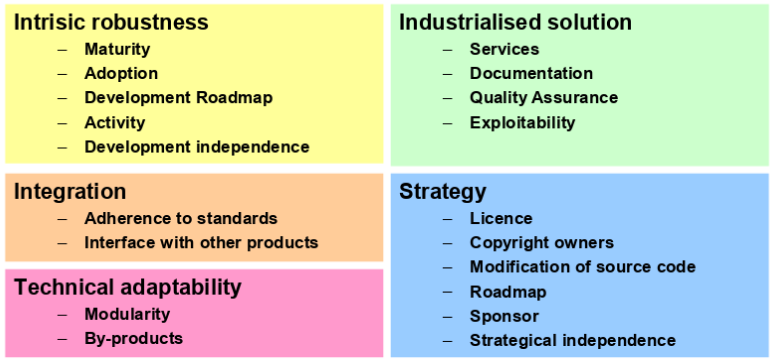
\includegraphics[height=6cm]{figs/qsos-risks}
  \end{center}  

\end{frame}


%%-----------------------------------------
\begin{frame}[fragile]
  \frametitle{QSOS}

  \begin{center}
  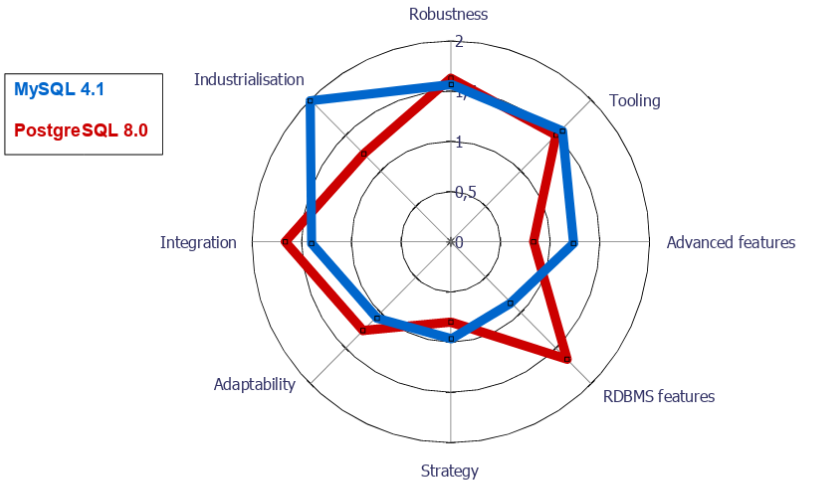
\includegraphics[height=6cm]{figs/qsos-example}
  \end{center}  

\end{frame}

%% %%-----------------------------------------
%% \begin{frame}[fragile]
%%   \frametitle{OMM}

%%   QualiPSo OpenSource Maturity Model
%% \end{frame}


%%-----------------------------------------
\begin{frame}[fragile]
  \frametitle{Polarsys Quality Model}

  \begin{center}
  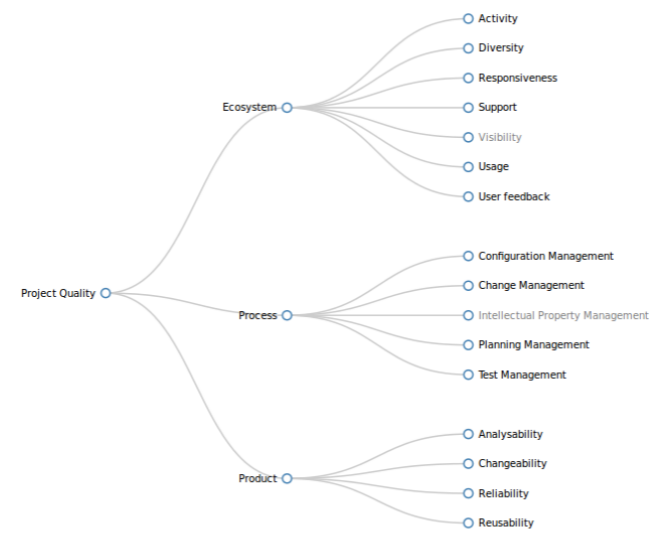
\includegraphics[height=6cm]{figs/polarsys-attributes}
  \end{center}  
  
\end{frame}

%%-----------------------------------------
\begin{frame}[fragile]
  \frametitle{Polarsys Quality Model}

  \begin{center}
  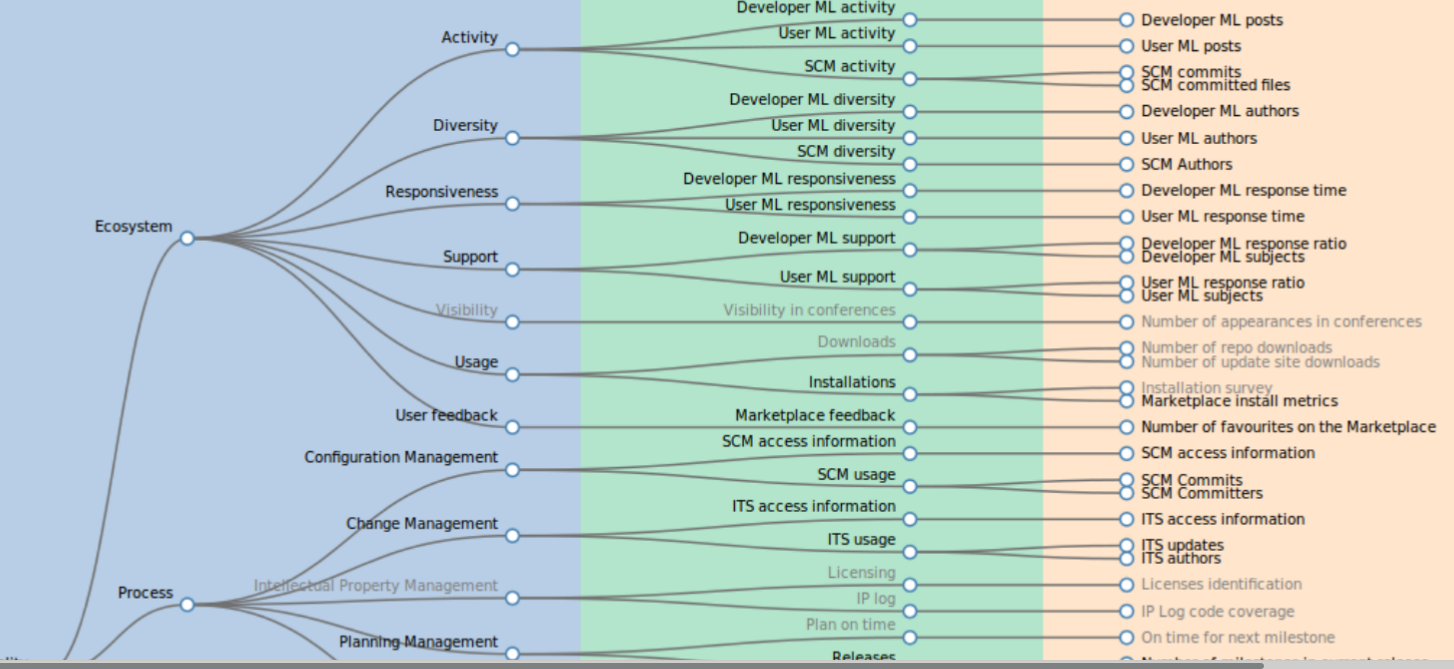
\includegraphics[height=5.5cm]{figs/polarsys-all}
  \end{center}  
  
\end{frame}

%%-----------------------------------------
%%-----------------------------------------
\section{Software health}

%%-----------------------------------------
\begin{frame}[fragile]

  
  {\em
    \begin{quote}
      ``A set of \textbf{characteristics} \\
      of a software \textbf{project} \\
      determining its capability for producing \\
      \textbf{software of good quality}, \\
      according to certain \textbf{criteria}
  \end{quote}
  }
  
\end{frame}


%%-----------------------------------------
\begin{frame}[fragile]
  \frametitle{What is software health?}

  A concept applied to a \textbf{project}:
  
  \begin{itemize}
  \item Criteria to define quality
  \item Characteristics that allow for that quality
  \item Time spot for measuring
  \end{itemize}
\end{frame}

%%-----------------------------------------
\begin{frame}[fragile]
  \frametitle{Measuring software health}

  \begin{itemize}
  \item Quantify quality criteria
  \item Find indicators that summarize criteria
  \item Find values for them that characterize health
  \item Track their evolution
  \end{itemize}
\end{frame}

%%-----------------------------------------
\begin{frame}[fragile]
  \frametitle{Example}

  \begin{itemize}
  \item Criteria for quality: minimize unfixed errors 
  \item Indicator: unfixed bug reports
  \item Healthy value: X unfixed bug reports per KLoC
  \item Alarm when number below X
  \end{itemize}
\end{frame}

%%-----------------------------------------
\begin{frame}[fragile]
  \frametitle{The causes for health}

  {\em
  The really interesting matter \\
  is to know the causes \\
  for variation in indicators \\
  }
  \vspace{.5cm}
  
  Example: unfixed bug reports are minimized by good code review
  
\end{frame}


%%-----------------------------------------
%%-----------------------------------------
\section{Some ideas}

%%-----------------------------------------
\begin{frame}[fragile]
  \frametitle{On the shoulders of giants}

  Systems are composed of many modules:

  \begin{itemize}
  \item Dependencies matter
  \item Overall health dependent on health of all components
  \item In some cases, dependent on health of the most unhealthy component
  \item Projects and communities are interdependent
  \end{itemize}

  Assessing the overall health of a complete system
  
\end{frame}

%%-----------------------------------------
\begin{frame}[fragile]
  \frametitle{Making decisions for tomorrow}

  Many systems are in production for many years:

  \begin{itemize}
  \item Prediction on future health
  \item Not all aspects are equally relevant \\
    (example: fixing bugs vs. new functionality)
  \item Important: understanding dynamics \\
    (extending past to future is not good enough)
  \end{itemize}
\end{frame}

%%-----------------------------------------
\begin{frame}[fragile]
  \frametitle{Integrating metrics with development}

  Can health be yet another factor to consider?

  \begin{itemize}
  \item It could be an indicator for every stakeholder
  \item Computed frequently, so that it is up to date
  \item Published widely, so that everyone is aware
  \end{itemize}

  Include health in the data for decision making

\end{frame}

%%-----------------------------------------
\begin{frame}[fragile]
  \frametitle{Working with stakeholders}

  \begin{itemize}
  \item Builders
  \item Integrators
  \item Users
  \end{itemize}

  \vspace{.5cm}

  \begin{flushright}
  Health for different actors \\
  for different purposes \\
  \end{flushright}
  
\end{frame}

%%-----------------------------------------
\begin{frame}[fragile]

  \begin{center}
  
\includegraphics[height=3.2cm]{figs/chaoss}
  \end{center}  

  \url{http://chaoss.community}
  
\end{frame}

%%-----------------------------------------
\begin{frame}[fragile]
  \frametitle{Understanding dynamics}

  How do specific actions impact \\
  on the health model \\
  for a software development system?
\end{frame}

%%-----------------------------------------
\begin{frame}[fragile]
  \frametitle{Towards a new research framework}

  Define health conditions \\
  Find out how to measure indicators of health \\
  Study deviations from healthy conditions \\
  Learn how to help to go back to healthy \\

  Include all of this in the development process
\end{frame}

%%-----------------------------------------
\begin{frame}[fragile]
  \frametitle{Simple example}

  Health condition: no regressions \\
  Indicators: tests failing \\
  Deviations: old errors appear \\
  Mitigation: automatic testing \\

  \begin{center}
    Continuous integration system
  \end{center}
\end{frame}

%%-----------------------------------------
\begin{frame}[fragile]
  \frametitle{Beyond opinions}

  Evidence that the indicator shows
  deviation from healthy condition

  \vspace{.5cm}
  
  Evidence of mitigation:

  \begin{itemize}
  \item condition go back to healthy
  \item indicator go back to normal
  \end{itemize}
  
\end{frame}

%%-----------------------------------------
%%-----------------------------------------
\section{Concluding...}

%%-----------------------------------------
\begin{frame}[fragile]

  {\Large
  \begin{center}
    Can we do this \\
    in non-trivial cases?
  \end{center}
  }
  
\end{frame}

%%-----------------------------------------
\begin{frame}[fragile]

  {\large
  \begin{center}
    Software health may provide \\
    a good framework \\
    for structuring research, \\
    producing useful analysis, \\
    and producing actionable outputs \\
  \end{center}
  }  
\end{frame}

%%-----------------------------------------
\frame{
~
\vspace{1cm}

\begin{flushright}


\includegraphics[width=2.2cm]{figs/by-sa}
 \\

\begin{footnotesize}
\copyright 2019 Jesus M. Gonzalez-Barahona. \\

\vspace{.4cm}

Some rights reserved. This document is distributed under the terms of the Creative Commons License ``Attribution-ShareAlike 4.0'',
available in \\
{\scriptsize \url{http://creativecommons.org/licenses/by-sa/4.0/}} \\

\vspace{.4cm}

This document (including source) is available from
\url{https://jgbarah.github.io/presentaciones}

\end{footnotesize}
\end{flushright}

}
%%

%\againframe{firstframe}

\end{document}
